%!TEX root = main_acm.tex

\section{Background}
\label{sec:back}

\subsection{BGP and Anycast}

Border Gateway Protocol (BGP) \cite{rekhter2005border} is the de facto
inter-domain routing protocol, designed to exchange reachability information
among autonomous systems on the Internet. BGP selects a best AS path based on various attributes (e.g., the shortest path) to reach the specific destination.

Anycast \cite{abley2006operation} is a network addressing and routing methodology by which a collection of servers announce the same IP address from multiple geographically distributed sites. 
As routers usually choose the shortest AS path, the user requests sent to an anycast address are routed to the topologically nearest endpoint. 
As a result, anycast has many advantages over unicast such as reduced latency, load balancing, DDoS mitigation, and improved robustness.

\subsection{Remote Peering}  
Peering is a relationship where two networks exchange traffic directly rather than through a transit provider.
Remote peering~\cite{castro2014remote, Nomikos18} is a new peering type where a
network peers at an IXP through layer-2 remote peering providers such as resellers without a physical presence in the IXP's infrastructure. Fig. \ref{RP} shows an example of remote peering. 
Remote peering can be implemented with standard methods like MPLS
(Multi-Protocol Label Switching) and VPNs (Virtual Private Networks) in layer-2,
and provide benefits such as low cost, increased connectivity, and easy
management. Nevertheless, it also has some drawbacks such as degradation of
performance, loss of resilience, and difficulty for layer-3 management~\cite{Nomikos18}.
Furthermore, due to the invisibility at layer-3, BGP routers are not aware of
remote peering and may select as the shortest path a route where the actual endpoints are far from one another.

\begin{figure}[thbp]
\centerline{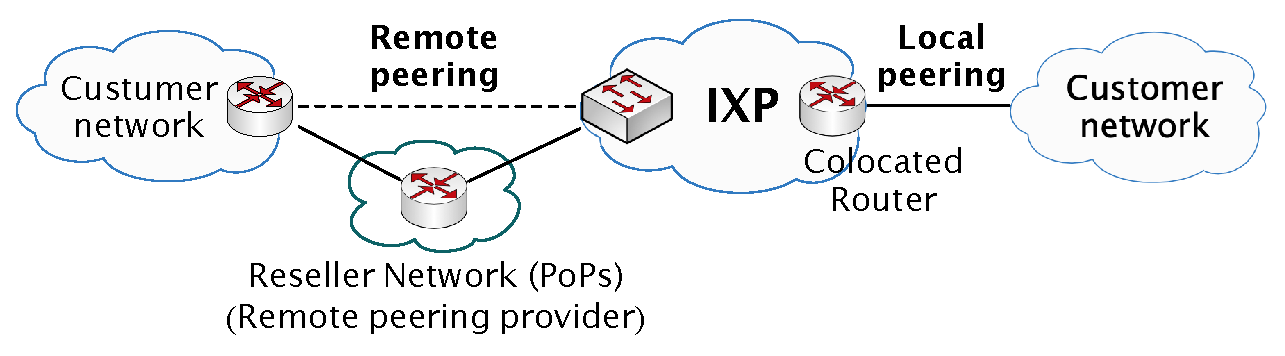
\includegraphics[scale=0.39]{fig/remote_peering.eps}}
\vspace{6pt}
\caption{Local and Remote Peering Models}
\label{RP}
\end{figure}
\vspace{-3pt}
